\documentclass[letter,11pt]{article}
\usepackage[margin=1.5cm]{geometry}
\usepackage{latexsym}
\usepackage{amsmath}
\usepackage{color}
\usepackage{graphicx}
\usepackage{amssymb}
\usepackage{alltt}
\usepackage{enumitem}
\usepackage{siunitx}
\usepackage{physics}
\usepackage{float}
\usepackage{bm}

\newenvironment{solution}{
    \vspace{0.16in} {\bf Solution:}
    
}{
	\vspace{0.16in}
}
\newcommand{\inti}[4]{
	\int_{#1}^{#2} #3 \, \mathrm{d} #4
}
\newcommand{\xx}{\bm{x}}
\newcommand{\mub}{\bm{\mu}}
\newcommand{\Sigmab}{\bm{\Sigma}}
\newcommand{\m}[1]{\begin{bmatrix}#1\end{bmatrix}}
\newcommand{\N}{\mathcal{N}}

%------------------------------------------------------

\begin{document}

\begin{center}
    {\bf \Large Math 189R problem set 4} \\
    \vspace{0.1in}
    Adam Guo \quad 2020-02-17
\end{center}

\begin{enumerate}
    \item \textbf{(Conditioning a Gaussian)} Note that from Murphy page 113.
    ``Equation 4.69 is of such importance in this book that we have put a box
    around it, so you can easily find it.'' That equation is important. Read
    through the proof of the result. Suppose we have a distribution over random
    variables $\xx = (\xx_1, \xx_2)$ that is jointly Gaussian with parameters

    \[\mub = \m{\mub_1 \\ \mub_2}, \quad
    \Sigmab = \m{\Sigmab_{11} & \Sigmab_{12} \\ \Sigmab_{21} & \Sigmab_{22}},\]
    where
    \[\mub_1 = \m{0 \\ 0}, \quad
    \mub_2 = 5, \quad
    \Sigmab_{11} = \m{6 & 8 \\ 8 & 13}, \quad
    \Sigmab_{21}^T = \Sigmab_{12} = \m{5 \\ 11}, \quad
    \Sigmab_{22} = \m{14}\]

    Compute
    \begin{enumerate}[label=(\alph*)]
        \item The marginal distribution $p(\xx_1)$.

        \begin{solution}
            \[p(\xx_1) = \N(\xx_1 \mid \mub_1, \Sigmab_{11})
            = \N\left(\m{0 \\ 0}, \m{6 & 8 \\ 8 & 13}\right)\]
        \end{solution}

        %------------------------------

        \item The marginal distribution $p(\xx_2)$.
        
        \begin{solution}
            \[p(\xx_2) = \N(\xx_2 \mid \mub_2, \Sigmab_{22}) = \N(5, 14)\]
        \end{solution}

        %------------------------------

        \item The conditional distribution $p(\xx_1 \mid \xx_2)$.
        
        \begin{solution}
            \begin{align*}
                p(\xx_1 \mid \xx_2) &= \N(\xx_1 \mid \mub_{1 \mid 2},
                                       \Sigmab_{1 \mid 2}) \\
                \mub_{1 \mid 2} &= \m{0 \\ 0} + \m{5 \\ 11} (1/14) (\xx_2 - 5) \\
                                &= \m{5 \\ 11} (1/14) (\xx_2 - 5) \\
                \Sigmab_{1 \mid 2} &= \m{6 & 8 \\ 8 & 13} - \m{5 \\ 11} (1/14)
                                      \m{5 & 11} \\
                                   &= \m{59/14 & 57/14 \\ 57/14 & 61/14} \\
                p(\xx_1 \mid \xx_2) &= \N\left(\m{5 \\ 11} (1/14) (\xx_2 - 5),
                                       \m{59/14 & 57/14 \\ 57/14 & 61/14}\right)
            \end{align*}
        \end{solution}

        %------------------------------
        
        \item The conditional distribution $p(\xx_2 \mid \xx_1)$.
        
        \begin{solution}
            \begin{align*}
                \mub_{2 \mid 1} &= 5 + \m{5 & 11} \m{6 & 8 \\ 8 & 13}^{-1}
                                   (\xx_1 - \m{0 \\ 0}) \\
                                &= 5 + \m{-23/14 & 13/7} \xx_1 \\
                \Sigmab_{2 \mid 1} &= 14 - \m{5 & 11} \m{6 & 8 \\ 8 & 13}^{-1}
                                      \m{5 \\ 11} \\
                                   &= 14 - 171/14 \\
                                   &= 25/14 \\
                p(\xx_2 \mid \xx_1) &= \N(5 + \m{-23/14 & 13/7} \xx_1, 25/14)
            \end{align*}
        \end{solution}
    \end{enumerate}

    \newpage

    %----------------------------------

    \item \textbf{(MNIST)} In this problem, we will use the MNIST dataset, a
    classic in the deep learning literature as a toy dataset to test algorithms
    on, to set up a model for logistic regression and softmax regression. In the
    starter code we have already parsed the data for you. However, you might
    need internet connection to access the data and therefore successfully run
    the starter code.
    
    The problem is this: we have images of handwritten digits with $28\times 28$
    pixels in each image, as well as the label of which digit $0 \leq
    \texttt{label} \leq 9$ the written digit corresponds to. Given a new image
    of a handwritten digit, we want to be able to predict which digit it is. The
    format of the data is \texttt{label, pix-11, pix-12, pix-13, ...} where
    \texttt{pix-ij} is the pixel in the \texttt{ith} row and \texttt{jth} column.

    \begin{enumerate}[label=(\alph*)]
        \item \textbf{(logistic)} Restrict the dataset to only the digits with a
        label of 0 or 1. Implement L2 regularized logistic regression as a model
        to compute $P(y=1\mid\xx)$ for a different value of the regularization
        parameter $\lambda$. Plot the learning curve (objective vs. iteration)
        when using Newton's Method \textit{and} gradient descent. Plot the
        accuracy, precision ($p = P(y=1 \mid \hat y=1)$), recall ($r = P(\hat
        y=1 \mid y=1)$), and F1-score ($F1 = 2pr / (p+r)$) for different values of
        $\lambda$ (try at least 10 different values including $\lambda = 0$) on
        the test set and report the value of $\lambda$ which maximizes the
        accuracy on the test set. What is your accuracy on the test set for this
        model? Your accuracy should definitely be over 90\%.

        \begin{solution}
            $\lambda = 5.0$ maximises the accuracy on the test set. Accuracy is
            around 0.9995.
            \begin{figure}[H]
                \centering
                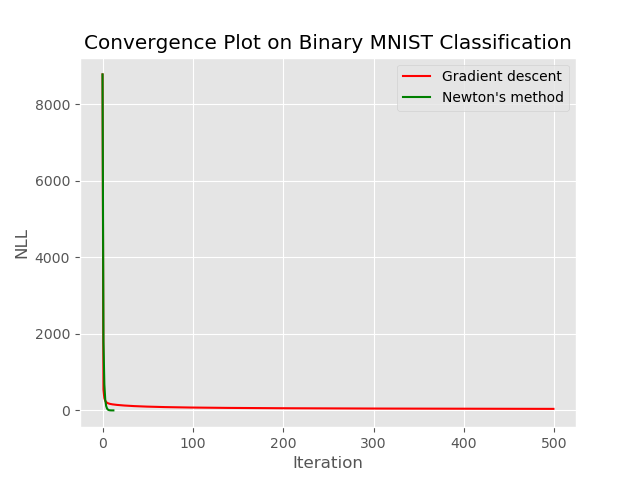
\includegraphics[width=9.5cm]{hw4pr2a_convergence.png}
            \end{figure}
            \begin{figure}[H]
                \centering
                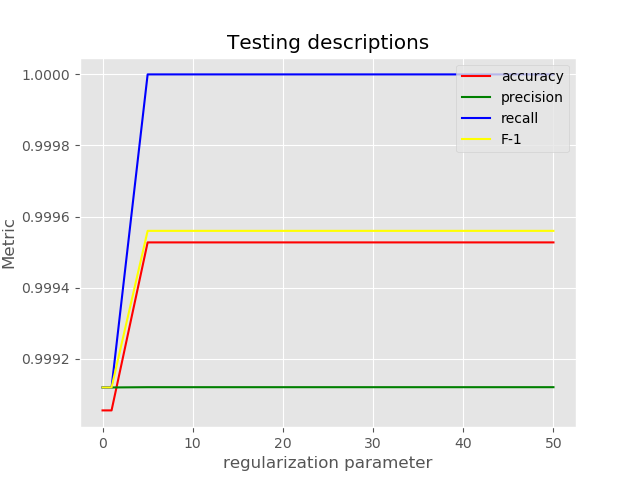
\includegraphics[width=9.5cm]{hw4pr2a_description.png}
            \end{figure}
        \end{solution}

        \item \textbf{(softmax)} Now we will use the whole dataset and predict the
        label of each digit using L2 regularized softmax regression (multinomial
        logistic regression). Implement this using gradient descent, and plot the
        accuracy on the test set for different values of $\lambda$, the
        regularization parameter. Report the test accuracy for the optimal value of
        $\lambda$ as well as its learning curve. Your accuracy should be over 90\%.
        
        \begin{solution}
            The optimal value of $\lambda$ is 0.01, which yields a test accuracy
            of 91.9\%.

            \begin{figure}[H]
                \centering
                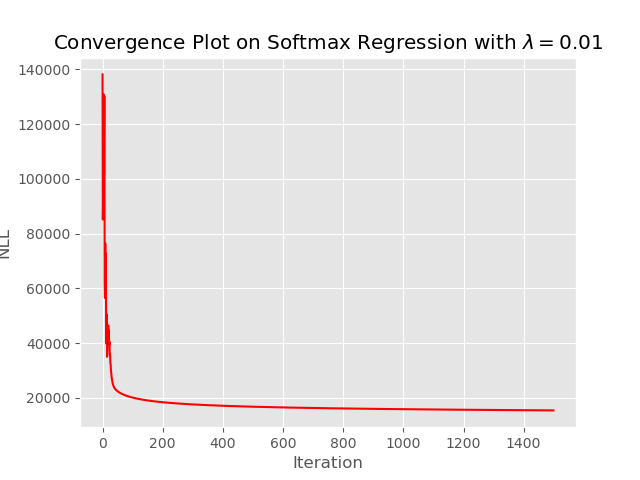
\includegraphics[width=9.5cm]{hw4pr2b_convergence.png}
            \end{figure}
            \begin{figure}[H]
                \centering
                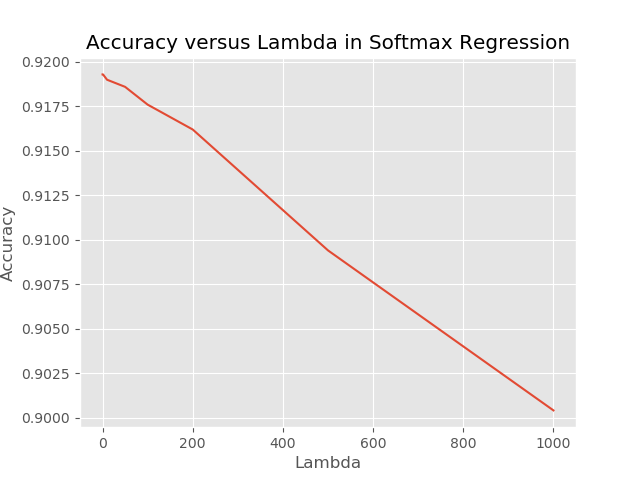
\includegraphics[width=9.5cm]{hw4pr2b_lva.png}
            \end{figure}
        \end{solution}
    \end{enumerate}
\end{enumerate}

\end{document}
